\chapter{Marco Metodológico}


\section{Metodología Tradicional} 
%%%%%%%%%%%%%%%%%%%%%%%%%%%%%%% RUP %%%%%%%%%%%%%%%%%%%%%%%%%%%%%%%%%%%
\subsection{RUP}

 RUP es un proceso para el desarrollo de un proyecto de software que define claramente quien, cómo, cuándo y qué debe hacerse en el proyecto, con 3 características esenciales, está dirigido por:

\begin{itemize}

    \item Los Casos de Uso : que orientan el proyecto a la importancia para el usuario y lo que este quiere. 

    \item La arquitectura: que Relaciona la toma de decisiones que indican cómo tiene que ser construido el sistema y en qué orden.

    \item Iterativo e incremental: dividiéndose el proyecto en mini proyectos donde los casos de uso y la arquitectura cumplen sus objetivos de manera más depurada.

\end{itemize}


\subsubsection{Ciclo de vida}
    RUP divide el proceso en 4 fases, dentro de las cuales se realizan varias iteraciones en número variable según el proyecto y en las que se hace un mayor o menor hincapié en los distintas actividades

\begin{figure}[H]
\begin{center}
	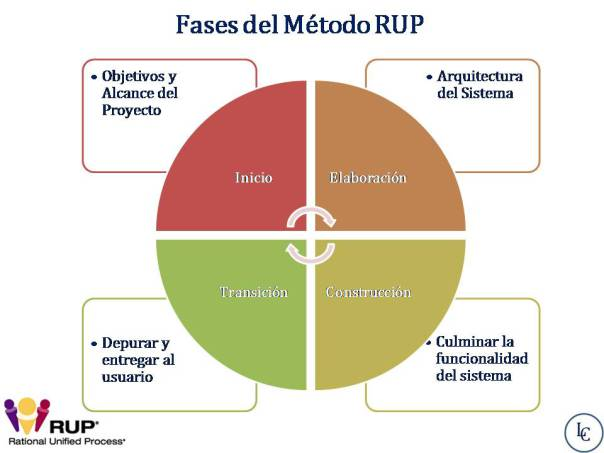
\includegraphics[width=13cm,height=8cm]{img/fases-rup.jpg}
\end{center}
\caption{Proceso RUP. (Tomada de , 2014)}
\label{fig:Rup}
\end{figure}
%https://dtyoc.com/tag/johana-vincze/



\begin{itemize}

    \item Fase de Inicio: Esta fase tiene como propósito definir y acordar el alcance del proyecto con los patrocinadores, identificar los riesgos asociados al proyecto, proponer una visión muy general de la arquitectura de software y producir el plan de las fases y el de iteraciones posteriores.

	\item Fase de elaboración: En la fase de elaboración se seleccionan los casos de uso que permiten definir la arquitectura base del sistema y se desarrollaran en esta fase, se realiza la especificación de los casos de uso seleccionados y el primer análisis del dominio del problema, se diseña la solución preliminar.

	\item Fase de Desarrollo: El propósito de esta fase es completar la funcionalidad del sistema, para ello se deben clarificar los requisitos pendientes, administrar los cambios de acuerdo a las evaluaciones realizados por los usuarios y se realizan las mejoras para el proyecto.

	\item Fase de Transición: El propósito de esta fase es asegurar que el software esté disponible para los usuarios finales, ajustar los errores y defectos encontrados en las pruebas de aceptación, capacitar a los usuarios y proveer el soporte técnico necesario. Se debe verificar que el producto cumpla con las especificaciones entregadas por las personas involucradas en el proyecto.	

\end{itemize}

%https://es.scribd.com/doc/7844685/CONCEPTOS-DE-RUP
%%%%%%%%%%%%%%%%%%%%%%%%%%%%%%% END RUP %%%%%%%%%%%%%%%%%%%%%%%%%%%%%%%%%%%

%%%%%%%%%%%%%%%%%%%%%%%%%%%%%%% Cascada %%%%%%%%%%%%%%%%%%%%%%%%%%%%%%%%%%%

\subsection{Cascada}

Modelo en Cascada, también llamado Lineal secuencial, es el enfoque metodológico que ordena rigurosamente las etapas del proceso para el desarrollo de software, de tal forma que el inicio de cada etapa debe esperar a la finalización de la etapa anterior. 

\subsubsection{Fases del Modelo}

\begin{figure}[H]
\begin{center}
	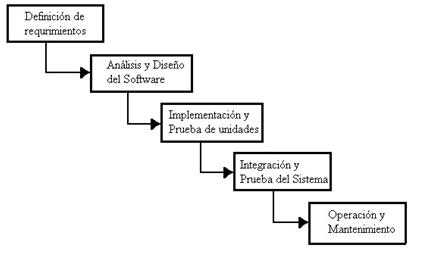
\includegraphics[width=13cm,height=8cm]{img/cascada.jpg}
\end{center}
\caption{Proceso Cascada. (Tomada de , 2014)}
\label{fig:Casacada}
\end{figure}

\begin{itemize}

    \item Análisis de requisitos: En esta fase se analizan las necesidades de los usuarios finales del software para determinar qué objetivos debe cubrir. De esta fase surge una memoria llamada SRD (documento de especificación de requisitos), que contiene la especificación completa de lo que debe hacer el sistema sin entrar en detalles internos. 

    %Es importante señalar que en esta etapa se debe consensuar todo lo que se requiere del sistema y será aquello 
    %lo que seguirá en las siguientes etapas, no pudiéndose requerir nuevos resultados a mitad del proceso de 
    %elaboración del software.

    \item Diseño del Sistema: Se descompone y organiza el sistema en elementos que puedan elaborarse por separado, aprovechando las ventajas del desarrollo en equipo. Como resultado surge el SDD (Documento de Diseño del Software), que contiene la descripción de la estructura relacional global del sistema y la especificación de lo que debe hacer cada una de sus partes, así como la manera en que se combinan unas con otras. 

    \item Diseño del Programa: Es la fase en donde se realizan los algoritmos necesarios para el cumplimiento de los requerimientos del usuario así como también los análisis necesarios para saber que herramientas usar en la etapa de Codificación.

    \item Codificación: Es la fase en donde se implementa el código fuente, haciendo uso de prototipos así como de pruebas y ensayos para corregir errores. Dependiendo del lenguaje de programación y su versión se crean las bibliotecas y componentes reutilizables dentro del mismo proyecto para hacer que la programación sea un proceso mucho más rápido.

    \item Pruebas: Los elementos, ya programados, se ensamblan para componer el sistema y se comprueba que funciona correctamente y que cumple con los requisitos, antes de ser entregado al usuario final.

    %Existen varios tipos de Pruebas:  Pruebas de unidad Pruebas de integración Pruebas de sistema Pruebas de %aceptación

    \item Verificación: Es la fase en donde el usuario final ejecuta el sistema, para ello el o los programadores ya realizaron exhaustivas pruebas para comprobar que el sistema no falle.

    \item Mantenimiento: Una de las etapas mas criticas, ya que se destina un 75 de los recursos, es el mantenimiento del Software ya que al utilizarlo como usuario final puede ser que no cumpla con todas nuestras expectativas.

    %Tipos de Mantenimiento: Preventivo y Perfectivo, Correctivo, Evolutivo

\end{itemize}

%http://www.ecured.cu/Modelo_en_cascada


%%%%%%%%%%%%%%%%%%%%%%%%%%%%%%% End Cascada %%%%%%%%%%%%%%%%%%%%%%%%%%%%%%%%%%%

\subsection{Cuadro Comparativo}

\begin{table}[H]	
\begin{center}
\begin{tabular}{ | m{6cm} | m{6cm} | } 
  \hline
 RUP & Casacada \\
 \hline
 Es un proceso iterativo.  & Es un proceso secuencial.  \\
 \hline
 Desarrolla el producto en base al feedback de los accionistas.  &   El proceso de creación del software tarda mucho tiempo ya que debe pasar por el proceso de prueba. \\
 \hline
  Cada iteracion produce una versión ejecutable. & Hasta que el software no esté completo no se opera. Esto es la base para que funcione bien. \\
 \hline
  Es un marco adaptable de procesos de software & Es un proceso concreto definido. \\
 \hline
\end{tabular}
\caption{Tabla comparativa de metodologías tradicionales}
\label{Tabla:1}
\end{center}
\end{table}	
.


\section{Metodología Ágil} 

El desarrollo ágil de software envuelve un enfoque para la toma de decisiones en los proyectos basados en el desarrollo iterativo e incremental, donde los requisitos y soluciones evolucionan con el tiempo según la necesidad del proyecto. Así el trabajo es realizado mediante la colaboración de equipos auto-organizados y multidisciplinarios, inmersos en un proceso compartido de toma de decisiones a corto plazo.

%%%%%%%%%%%%%%%%%%%%%%%%%%%%%%% Scrum %%%%%%%%%%%%%%%%%%%%%%%%%%%%%%%%%%%

\subsection{SCRUM}
\subsubsection{Ciclo de vida}

\begin{center}
	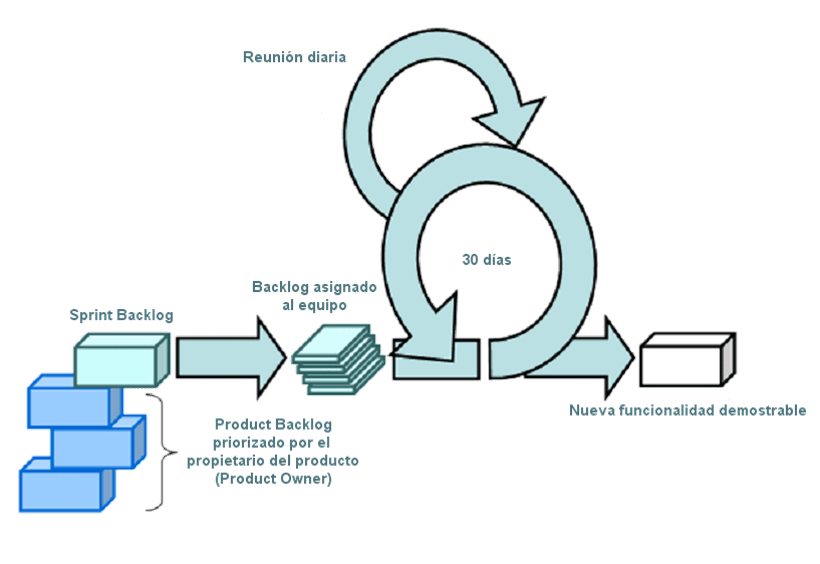
\includegraphics[width=13cm,height=8cm]{img/scrum.png}
\end{center}

\subsubsection{Spring}
\setlength{\parskip}{5mm}

	Es el periodo de tiempo durante el que se desarrolla un incremento de funcionalidad dura máximo 30 días. Constituye el núcleo de Scrum, que divide de esta forma el desarrollo de un proyecto en un conjunto de pequeñas “carreras”. Durante el proceso no se puede modificar el trabajo que se ha acordado en el Backlog, solo es posible cambiar el curso de un sprint abortándolo y esto solo puede hacerlo el Scrum Master. 
	
\setlength{\parskip}{0mm}

\subsubsection{Planificación del sprint}
\setlength{\parskip}{5mm}

	En esta reunión se toman como base las prioridades y necesidades de negocio del cliente, y se determinan cuáles y cómo van a ser las funcionalidades que se incorporarán al producto en el siguiente sprint. Se trata de  una reunión conducida por  el responsable del funcionamiento  del marco scrum (Scrum Master en scrum técnico, o un miembro del equipo,en scrum pragmático) a la que deben asistir el propietario del producto y el equipo completo, y a la que también pueden asistir otros implicados en el proyecto.

	La reunión puede durar una jornada de trabajo completa, cuando se trata de planificar un sprint largo (de un mes de duración) o un tiempo proporcional para planificar un sprint más breve. Esta reunión debe dar respuesta a dos cuestiones:

	\begin{itemize}
		\item Qué se entregará al terminar el sprint.

		\item Cuál es el trabajo necesario para realizar el incremento previsto, y cómo lo llevará a cabo el equipo.
	\end{itemize}

\setlength{\parskip}{0mm}
	La  reunión  se  articula  en  dos  partes  de  igual  duración,  para  dar  respuesta  a  una  de  estas  cuestiones,en cada una.
	
\setlength{\parskip}{0mm}

\subsubsection{Scrum diario}
\setlength{\parskip}{5mm}

	Reunión diaria breve, de no más de 15 minutos, en la que el equipo sincroniza el trabajo y establece el plan para las 24 horas siguientes. Informa el avance de cada miembro del equipo e identifica posible necesidades e impedimentos.
	
\setlength{\parskip}{0mm}

\subsubsection{Revisión de las Iteraciones}
\setlength{\parskip}{5mm}

	Al finalizar cada sprint se revisa funcionalmente el resultado, con todos los implicados en el proyecto. Es por tanto la duración del sprint, el período de tiempo máximo para descubrir planteamientos erróneos, mejorables o malinterpretaciones en las funcionalidades del producto.
	
\setlength{\parskip}{0mm}


\subsubsection{Retrospectiva}
\setlength{\parskip}{5mm}

	Reunión que se realiza tras la revisión de cada sprint, y antes de la reunión de planificación del siguiente, con una duración recomendada de una a tres horas, según la duración del sprint terminado.En ella el equipo realiza autoanálisis de su sobre su forma de trabajar, e identifica fortalezas y  puntos débiles. El objetivo es consolidar y afianzar las primeras, y planificar acciones de mejora sobre los segundos.

	El objetivo de la revisión del sprint es analizar “QUÉ” se está construyendo, mientras que una reunión retrospectiva se centra en “CÓMO” lo estamos construyendo: “CÓMO” estamos trabajando, con el objetivo de analizar problemas y aspectos mejorables.

	Las reuniones "retrospectivas" realizadas de forma periódica por el equipo para mejorar la forma de trabajo, se consideran cada vez más un componente del marco técnico de scrum, si bien no es una reunión para seguimiento de la evolución del producto, sino para mejora del marco de trabajo.
	
	(Juan Palacio,2014)
\setlength{\parskip}{0mm}

%http://www.scrummanager.net/files/sm_proyecto.pdf
%%%%%%%%%%%%%%%%%%%%%%%%%%%%%%% END Scrum %%%%%%%%%%%%%%%%%%%%%%%%%%%%%%%%%%%
    

%%%%%%%%%%%%%%%%%%%%%%%%%%%%%%% XP %%%%%%%%%%%%%%%%%%%%%%%%%%%%%%%%%%%
\subsection{XP}
\setlength{\parskip}{5mm}
Es una metodología ágil centrada en potenciar las relaciones interpersonales como clave para el éxito en desarrollo de software, promoviendo el trabajo en equipo, preocupándose por el aprendizaje de los desarrolladores, y propiciando un buen clima de trabajo. XP se basa en realimentación continua entre el cliente y el equipo de desarrollo, comunicación fluida entre todos los participantes, simplicidad en las soluciones implementadas y coraje para enfrentar los cambios. XP se define como especialmente adecuada para proyectos con requisitos imprecisos, muy cambiantes, y donde existe un alto riesgo técnico.
\setlength{\parskip}{0mm}
\subsubsection{Prácticas básicas de la programación extrema}
\setlength{\parskip}{5mm}

\begin{itemize}

    \item Equipo completo: Forman parte del equipo todas las personas que tienen algo que ver con el proyecto, incluido el cliente y el responsable del proyecto. 

	\item Planificación: Se hacen las historias de usuario y se planifica en qué orden se van a hacer y las mini-versiones. La planificación se revisa continuamente. 
	
	\item Test del cliente: El cliente, con la ayuda de los desarrolladores, propone sus propias pruebas para validar las mini-versiones. 

	\item Versiones pequeñas: Las mini-versiones deben ser lo suficientemente pequeñas como para poder hacer una cada pocas semanas. Deben ser versiones que ofrezcan algo útil al usuario final y no trozos de código que no pueda ver funcionando. 

	\item Diseño simple: Hacer siempre lo mínimo imprescindible de la forma más sencilla posible. Mantener siempre sencillo el código. 

	\item Pareja de programadores: Los programadores trabajan por parejas (dos delante del mismo ordenador) y se intercambian las parejas con frecuencia (un cambio diario). 

	\item Desarrollo guiado por las pruebas automáticas: Se deben realizar programas de prueba automática y deben ejecutarse con mucha frecuencia. Cuantas más pruebas se hagan, mejor. 

	\item Integración continua: Deben tenerse siempre un ejecutable del proyecto que funcione y en cuanto se tenga una nueva pequeña funcionalidad, debe recompilarse y probarse. Es un error mantener una versión congelada dos meses mientras se hacen mejoras y luego integrarlas todas de golpe. Cuando falle algo, no se sabe qué es lo que falla de todo lo que hemos metido. 

	\item El código es de todos: Cualquiera puede y debe tocar y conocer cualquier parte del código. Para eso se hacen las pruebas automáticas. 

	\item Normas de codificación: Debe haber un estilo común de codificación (no importa cual), de forma que parezca que ha sido realizado por una única persona. 

	\item Metáforas: Hay que buscar unas frases o nombres que definan cómo funcionan las distintas partes del programa, de forma que sólo con los nombres se pueda uno hacer una idea de qué es lo que hace cada parte del programa. Un ejemplo claro es el "recolector de basura" de java. Ayuda a que todos los programadores (y el cliente) sepan de qué estamos hablando y que no haya mal entendidos. 

	\item Ritmo sostenible: Se debe trabajar a un ritmo que se pueda mantener indefinidamente. Esto quiere decir que no debe haber días muertos en que no se sabe qué hacer y que no se deben hacer un exceso de horas otros días. Al tener claro semana a semana lo que debe hacerse, hay que trabajar duro en ello para conseguir el objetivo cercano de terminar una historia de usuario o mini-versión. 


\end{itemize}
\setlength{\parskip}{0mm}
\subsubsection{Ciclo de vida}
\setlength{\parskip}{5mm}
Un proyecto XP tiene éxito cuando el cliente selecciona el valor de negocio a implementar basado en la habilidad del equipo para medir la funcionalidad que puede entregar a través del tiempo. El ciclo de desarrollo consiste (a grandes rasgos) en los siguientes pasos:

\begin{itemize}

	\item El cliente define el valor de negocio a implementar.

	\item El programador estima el esfuerzo necesario para su implementación.

	\item El cliente selecciona qué construir, de acuerdo con sus prioridades y las restricciones de tiempo.

	\item El programador construye ese valor de negocio.

	\item Vuelve al paso 1.

\end{itemize}
    
En todas las iteraciones de este ciclo tanto el cliente como el programador aprenden. No se debe presionar al programador a realizar más trabajo que el estimado, ya que se perderá calidad en el software o no se cumplirán los plazos. De la misma forma el cliente tiene la obligación de manejar el ámbito de entrega del producto, para asegurarse que el sistema tenga el mayor valor de negocio posible con cada iteración.

El ciclo de vida ideal de XP consiste de seis fases: % Exploración, Planificación de la Entrega (Release), Iteraciones, Producción, Mantenimiento y Muerte del Proyecto.



\setlength{\parskip}{0mm}


% http://ingenieriadesoftware.mex.tl/images/18149/PROGRAMACI%C3%93N%20EXTREMA.pdf
%%%%%%%%%%%%%%%%%%%%%%%%%%%%%%% END XP %%%%%%%%%%%%%%%%%%%%%%%%%%%%%%%%%%%

%%%%%%%%%%%%%%%%%%%%%%%%%%%%%%% Agilus %%%%%%%%%%%%%%%%%%%%%%%%%%%%%%%%%%%

\subsection{Agilus}
\setlength{\parskip}{5mm}

	El Método AgilUs es un método de desarrollo ágil, resultado de una de las líneas de investigación desarrolladas en el Centro de Ingeniería de Software y Sistemas (ISYS) de la Escuela de Computación, Universidad Central de Venezuela. Se basa en el concepto de usabilidad, en la necesidad de desarrollar software usables. Se fundamenta en el análisis centrado en el usuario y en la participación de especialistas, con el objetivo de evolucionar el software, a fin de que éste alcance el mayor grado de usabilidad una vez culminado su desarrollo. AgilUs es un método de desarrollo iterativo e incremental que pone el mayor peso del desarrollo en la consecución de la usabilidad. Se centra en que la construcción y desarrollo de las interfaces de usuario no debe ser una adición estética que se da al final del desarrollo del sistema sino, muy por el contrario, el desarrollo de interfaces de usuario debe guiar las decisiones en Ingeniería de Software. En AgilUs son los usuarios, y no el cliente ni los programadores quienes guían el desarrollo del proyecto.

	El Método AgilUs busca proporcionar un conjunto de actividades organizadas para construir la usabilidad en el diseño de interfaces de usuario durante el desarrollo de un producto de software. El proceso de desarrollo de software engloba las actividades de requisitos, análisis, prototipaje y entrega; así como las evaluaciones de usabilidad correspondientes a cada etapa del proceso. Se realizan en ciclos iterativos hasta alcanzar el producto final. En cada etapa del proceso de desarrollo de software, se incluyen actividades propias para la construcción de la usabilidad.

\setlength{\parskip}{0mm}

\subsubsection{Ciclo de vida}

	El ciclo de vida de AgilUs hace énfasis en la importancia del usuario y sus evaluaciones. Está basado en el desarrollo iterativo e incremental de prototipos de alta fidelidad hasta que se convierten en el producto final para entrega. Este producto final puede ser posteriormente modificado a través de un mantenimiento correctivo y/o evolutivo, que no está contemplado como parte del método.

\begin{figure}[H]
\begin{center}
	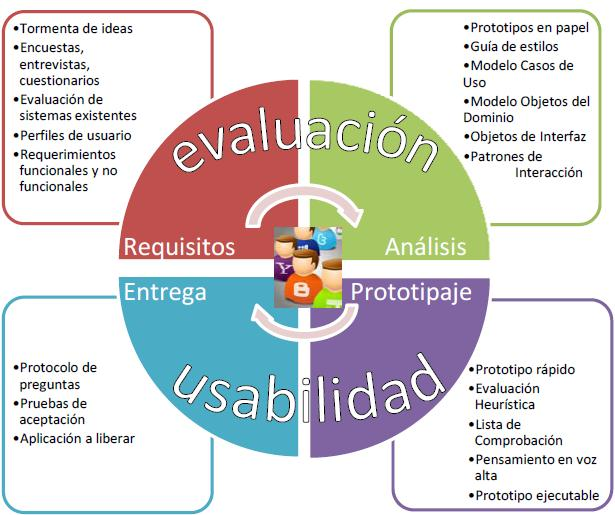
\includegraphics[width=13cm,height=8cm]{img/agilus.jpg}
\end{center}
\caption{El método AgilUs: etapas, actividades y artefactos.}
\label{fig:Rup}
\end{figure}
%https://dtyoc.com/tag/johana-vincze/



\begin{itemize}

    \item Requisitos: Se realiza el análisis global del problema a solucionar, se estudian productos similares existes, se genera un perfil de usuario, y se define la lista de requerimientos a desarrollar. Esta etapa es importante en el desarrollo del software, ya que un mal análisis de requisitos traería como consecuencia un software que no cumple con las necesidades del usuario.

    \item Análisis: Se lleva a cabo el análisis de la solución a desarrollar, se emplean diagramas de casos de uso y modelo de objetos del dominio, siguiendo la notación UML, para definir las funcionalidades que tendrá el producto a desarrollar.

    \item Prototipaje: Se implementa un prototipo rápido de la interfaz de usuario a partir de los patrones de interacción, el cual va evolucionando hasta convertirse en el producto final, se genera la guía de estilo, y se realizan evaluaciones de usabilidad apropiadas a esta etapa: las evaluaciones heurísticas y las listas de comprobación.

    \item Entrega: Se aplican las pruebas al sistema para certificar que la aplicación desarrollada sea un software usable y sin errores, finalmente se pone en producción la aplicación.

\end{itemize}

(\citet{agilusbib}, 2011) 

\subsection{Cuadro Comparativo}


\begin{table}[H]	
\begin{center}
\begin{tabular}{ | m{4cm} | m{4cm}| m{4cm}| } 
 \hline
 Scrum & XP & Agilus \\
 \hline
 val1. & val2. & val3.\\
 \hline
 val4. & val5. & val6.\\
 \hline
\end{tabular}
\caption{Tabla comparativa de metodologías ágiles}
\label{Tabla:2}
\end{center}
\end{table}	







\section{Cuadro comparativo [Metodologías Tradicionales vs Ágiles]} 

%%%%%%%%%%%%%%%%%%%%%%%%%%%%%%% END Agilus %%%%%%%%%%%%%%%%%%%%%%%%%%%%%%%%%%%
\begin{table}[H]	
\begin{center}
\begin{tabular}{ | m{6cm} | m{6cm} | } 
 \hline
 Tradicionales & Ágiles \\ 
	\hline
	Basadas en normas provenientes de estándares seguidos por el entorno de desarrollo.  Posee cierta resistencia a los cambios. 
	&
	Basadas en heurísticas provenientes de prácticas de producción de código las cuales previenen cambios durante el proyecto.\\ 
 	\hline
 	Define un proceso mucho más controlado junto con numerosas políticas/normas.
	&
	Define un proceso menos controlado, con pocos principios.\\ 
	\hline
	El cliente interactúa con el equipo de desarrollo mediante reuniones.	
	&
	El cliente es parte del equipo de desarrollo. \\ 
	\hline
	Genera más artefactos.	
	&
	Genera pocos artefactos.\\ 
	\hline

	Más roles.	
	&
	Pocos roles.\\ 
	\hline

	Grupos grandes y posiblemente distribuidos.	
	&
	Grupos pequeños (<10 integrantes) y trabajando en el mismo sitio.\\ 
	\hline

	Dependencia de la arquitectura de software mediante modelos.	
	& 
	Menor dependencia de la arquitectura de software.\\ 
	\hline

	Existe un contrato prefijado.	
	&
	No existe contrato tradicional o al menos es bastante flexible.\\ 
	\hline

\end{tabular}
\caption{Diferencias entre metodologías ágiles y tradicionales}
\label{Tabla:3}
\end{center}
\end{table}	

%https://es.scribd.com/doc/91676941/Metodologias-agiles-vs-tradicionales
%http://rdsoporteymantenimientodepc.blogspot.com/2014/03/metodologias-de-desarrollo-agiles-vs.html

